\documentclass[12pt,a4paper]{article}
\usepackage[utf8]{inputenc}
\usepackage[T1]{fontenc}
\usepackage[french]{babel}
\usepackage{geometry}
\usepackage{hyperref}
\usepackage{listings}
\usepackage{xcolor}
\usepackage{graphicx}
\usepackage{float}
\usepackage{pdflscape}
\usepackage{pdfpages} % Pour inclure les diagrammes pleine page sans distorsion

\geometry{margin=2.5cm}

\definecolor{codegreen}{rgb}{0,0.6,0}
\definecolor{codegray}{rgb}{0.5,0.5,0.5}
\definecolor{codepurple}{rgb}{0.58,0,0.82}
\definecolor{backcolour}{rgb}{0.95,0.95,0.92}

\lstdefinestyle{mystyle}{
    backgroundcolor=\color{backcolour},   
    commentstyle=\color{codegreen},
    keywordstyle=\color{magenta},
    numberstyle=\tiny\color{codegray},
    stringstyle=\color{codepurple},
    basicstyle=\ttfamily\footnotesize,
    breakatwhitespace=false,         
    breaklines=true,                 
    captionpos=b,                    
    keepspaces=true,                 
    numbers=left,                    
    numbersep=5pt,                  
    showspaces=false,                
    showstringspaces=false,
    showtabs=false,                  
    tabsize=2
}
\lstset{style=mystyle}

\begin{titlepage}
    \centering % Indispensable pour centrer le texte et les lignes
    \vspace*{2cm} % Ajoute un espace en haut pour ne pas coller au bord
    
    {\scshape\LARGE École Nationale des Sciences Appliquées de Tétouan} \\[0.8cm]
    {\large Filière : Cycle d'Ingénieur en Génie Informatique S6} \\[3cm] % Espace généreux avant le titre
    
    \rule{\linewidth}{0.5mm} \\[0.6cm] % \rule est plus facile à contrôler que \hrule
    {\huge\bfseries Application de Messagerie Instantanée \\[0.2cm] avec appels audio et vidéo} \\[0.5cm]
    \rule{\linewidth}{0.5mm} \\[3cm] % Espace généreux après le titre
    
    \begin{minipage}{0.45\textwidth}
        \begin{flushleft} \large
            \emph{Réalisé par :}\\[0.4cm]
            Abdellah \textbf{BOUARGUAN} \\[0.15cm]
            Nizar \textbf{BEN YACOUB}\\[0.15cm]
            Marouane \textbf{EL GHAZOUANI} \\[0.15cm]
            Nafissa \textbf{EL YOUNOUSSI} \\[0.15cm]
            Leila \textbf{BOUALAM} 
        \end{flushleft}
    \end{minipage}
    \hfill
    \\[0.8cm]
    \begin{minipage}{0.45\textwidth}
        \begin{flushright} \large
            \emph{Sous la direction de :}\\[0.4cm]
            Pr. \textsc{El Bouhdidi} Jaber
        \end{flushright}
    \end{minipage}
    
    \vfill % Ce vfill va agir comme un ressort et pousser la date tout en bas
    
    {\large \today}
    \vspace*{1cm} % Évite que la date soit coupée par l'imprimante en bas de page
\end{titlepage}

\begin{document}

\maketitle
\thispagestyle{empty}

\newpage
\tableofcontents
\newpage

\section{Introduction}
Ce document présente l'architecture logicielle et les choix de conception d'une application de messagerie instantanée, conçue pour simuler les fonctionnalités de base de WhatsApp. L'objectif principal de ce projet est de mettre en œuvre les concepts fondamentaux de la programmation orientée objet et de la conception UML, au travers d'une architecture client-serveur robuste et multi-threadée. L'application repose sur l'utilisation avancée des threads et des sockets réseaux (TCP et UDP), permettant une communication fluide en temps réel. L'interface utilisateur est développée à l'aide du framework JavaFX, offrant une expérience moderne et réactive. L'architecture est clairement séparée entre les composants client et serveur. Les fonctionnalités incluent l'authentification, le suivi de présence en temps réel, l'échange de messages textuels, et les communications multimédias (appels audio/vidéo) en Peer-to-Peer. Le serveur agit comme un routeur central utilisant des sockets TCP standards, tandis que les données de l'application sont persistées au sein d'une base de données PostgreSQL via JDBC.

\section{Analyse et Conception (UML)}
La conception du système a été modélisée en respectant rigoureusement les standards UML. Pour assurer une lisibilité optimale, les diagrammes complexes sont présentés sur des pages dédiées en pleine page.

\subsection{Cas d'Utilisation}
Le système interagit principalement avec l'Utilisateur final et un acteur système secondaire, la Base de données.

\begin{figure}[H]
    \centering
    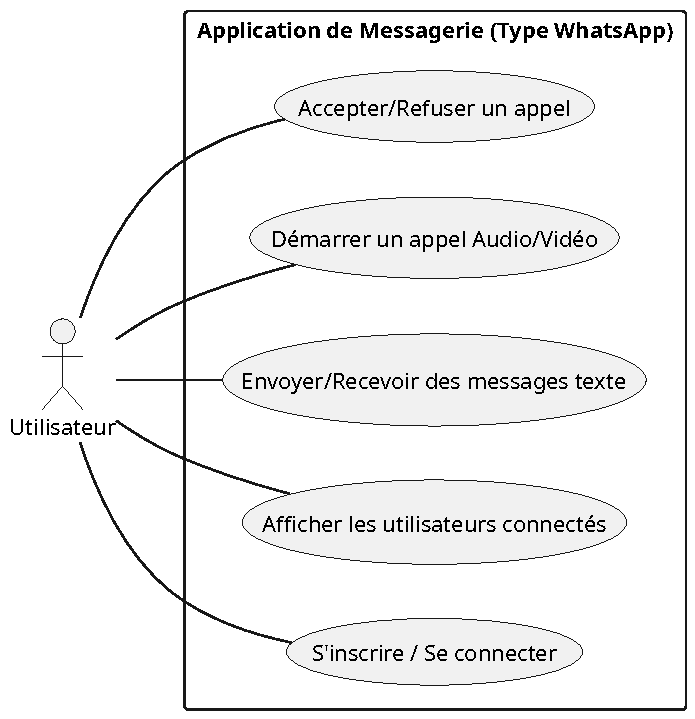
\includegraphics[width=0.9\textwidth]{../output/diagramme_cas_utilisation.pdf}
    \caption{Diagramme des Cas d'Utilisation du système}
\end{figure}

% On force l'inclusion des diagrammes larges sur des pages dédiées via pdfpages
% Cela permet de conserver la qualité vectorielle tout en utilisant tout l'espace disponible.

\newpage
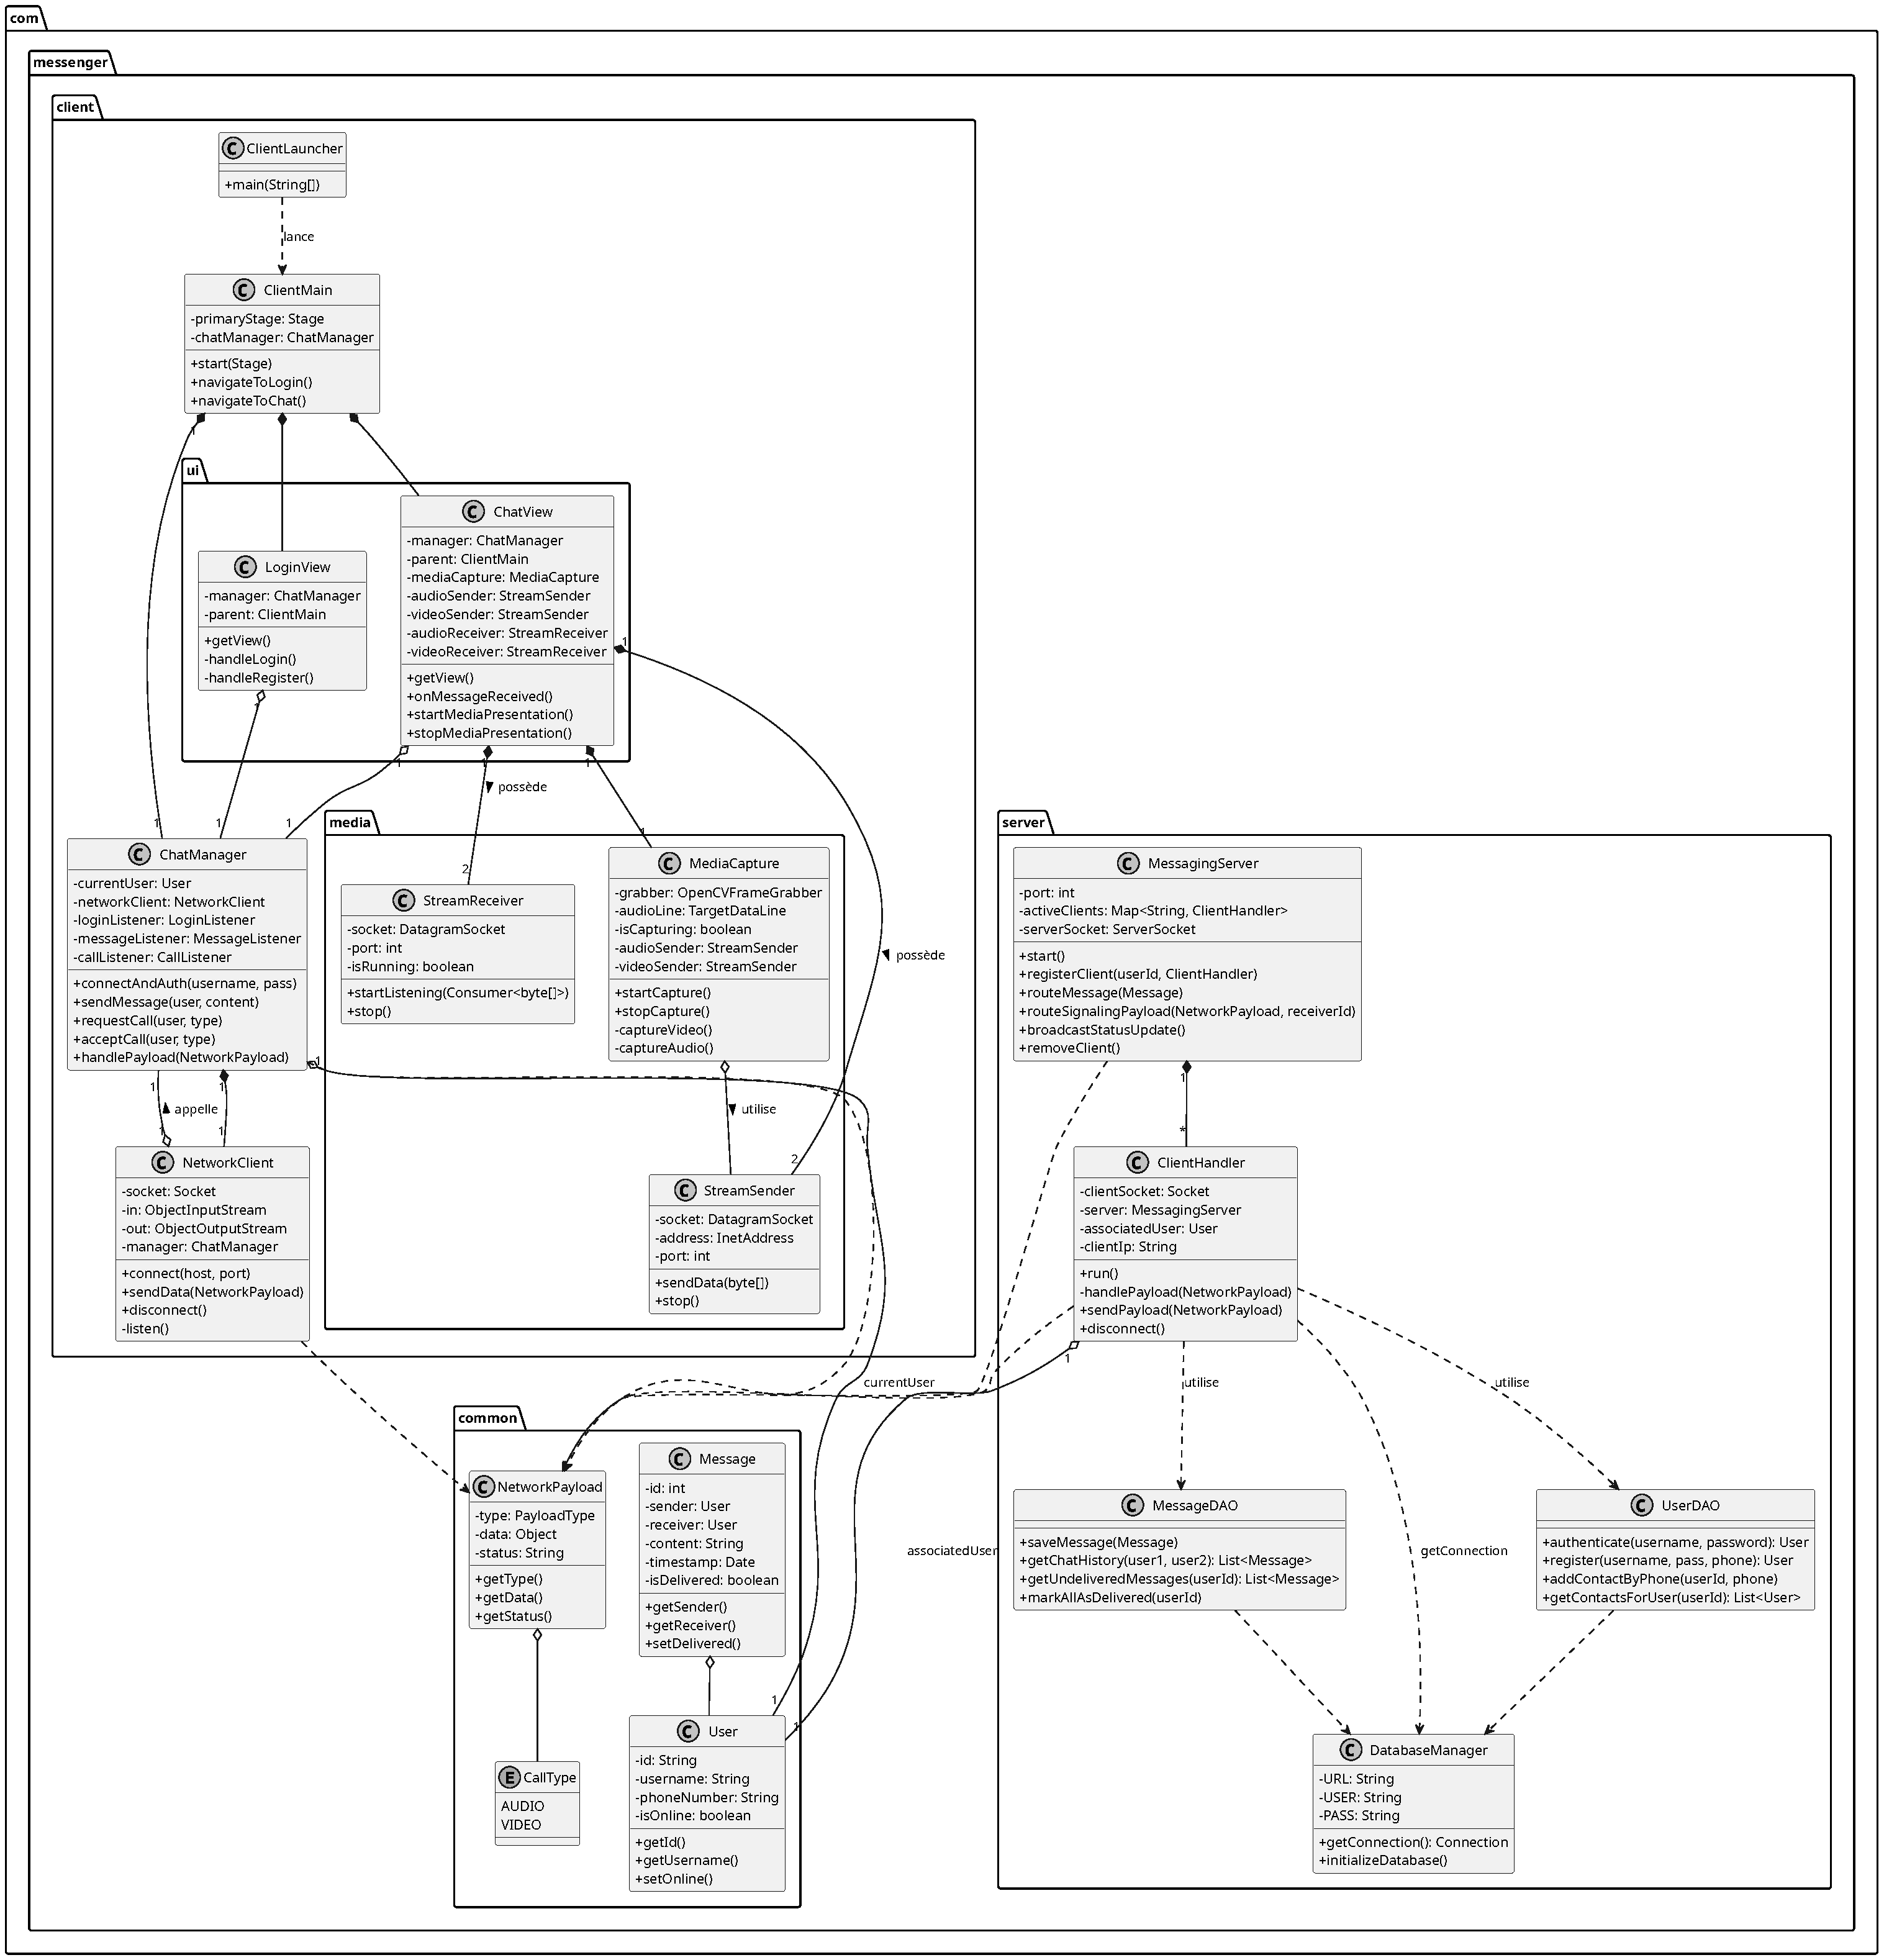
\includepdf[pages=-, landscape=true, pagecommand={\subsection{Diagramme de Classes}\label{sec:classes}}, scale=1]{../output/diagramme_classes.pdf}

\newpage
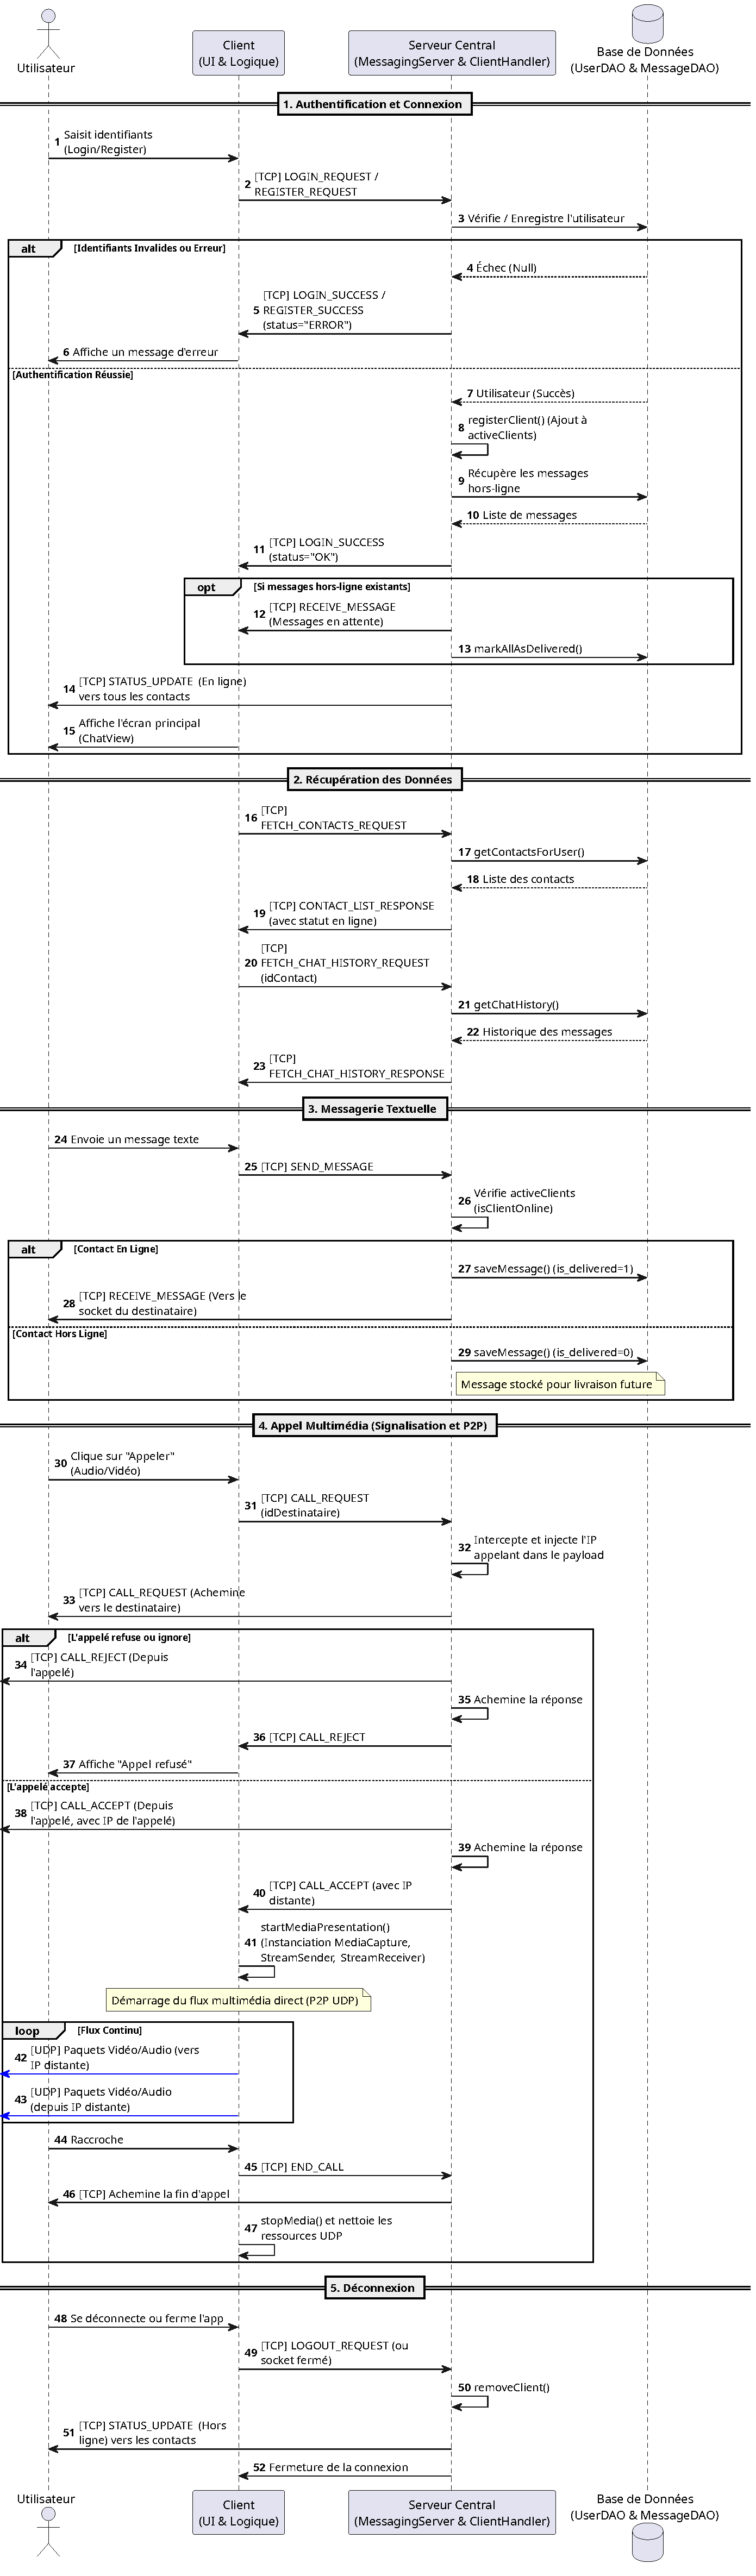
\includepdf[pages=-, landscape=true, pagecommand={\subsection{Diagramme de Séquence}\label{sec:sequence}}, scale=1]{../output/diagramme_sequence.pdf}

\newpage
\subsection{Diagramme de Déploiement}
Ce diagramme illustre la topologie physique du réseau et les protocoles de communication.

\begin{figure}[H]
    \centering
    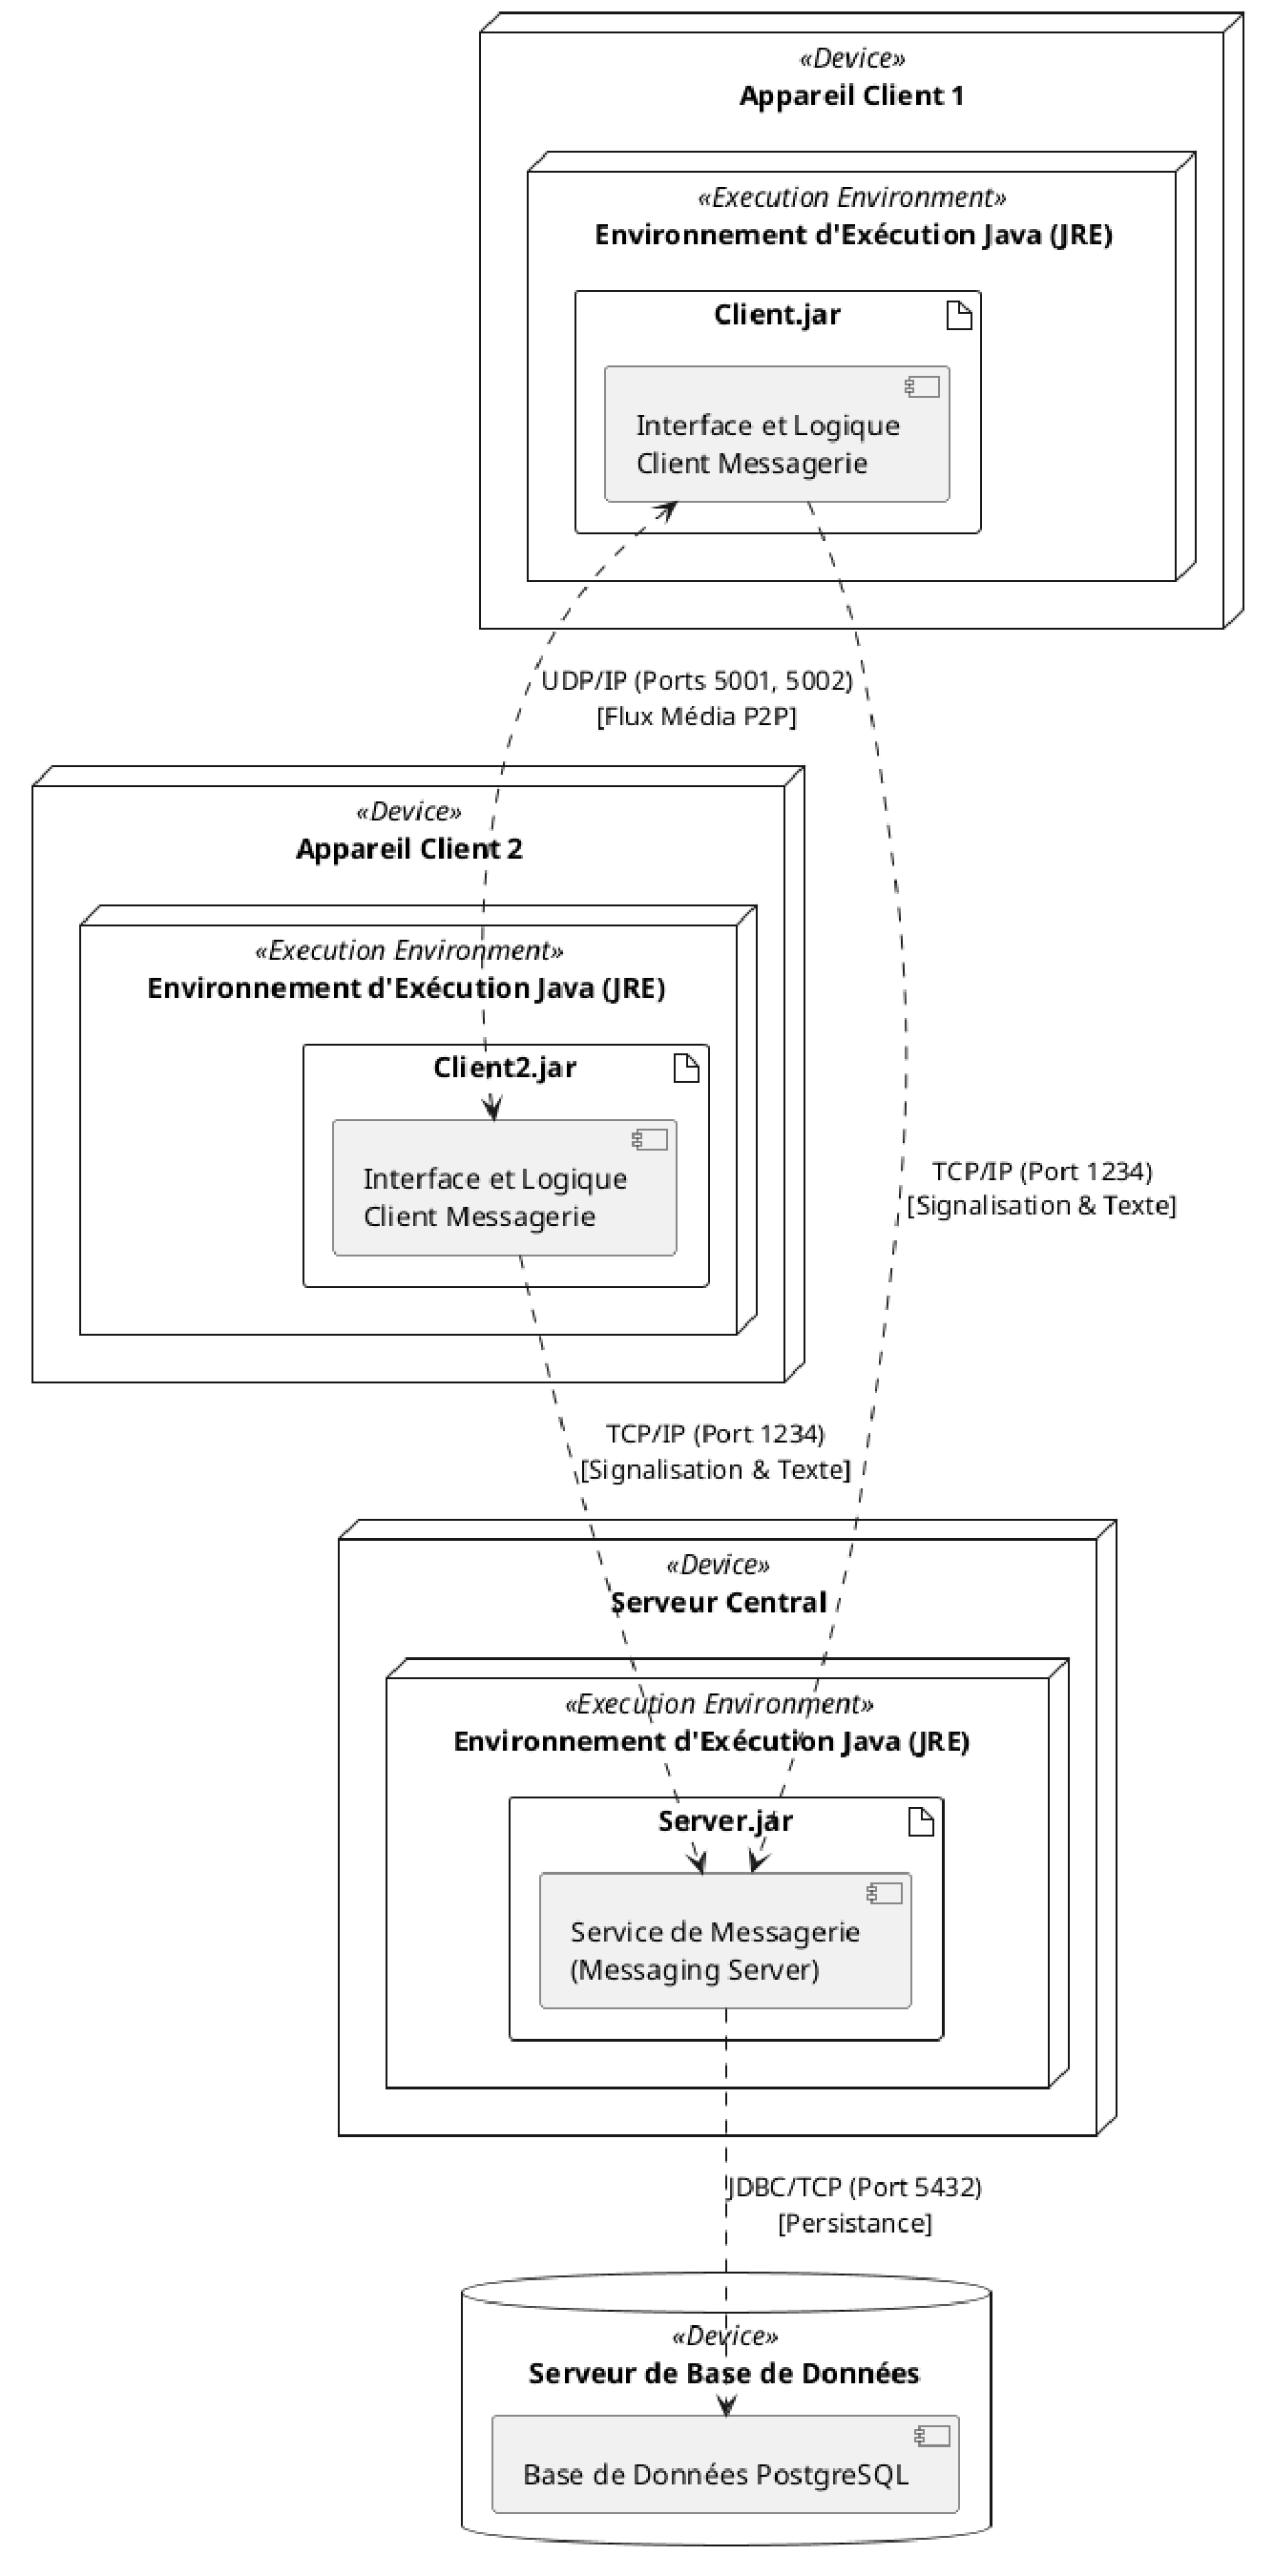
\includegraphics[width=0.9\textwidth]{../output/diagramme_deploiement.pdf}
    \caption{Diagramme de Déploiement}
\end{figure}

\section{Analyse des Modules (Architecture Technique)}

\subsection{Module Commun (\texttt{com.messenger.common})}
Le package \texttt{common} agit comme la couche de données fondamentale partagée entre le client et le serveur.
\begin{itemize}
    \item \texttt{User.java} \& \texttt{Message.java} : Ce sont des POJO standards implémentant l'interface \texttt{Serializable}.
    \item \texttt{CallType.java} : Une énumération définissant les types d'appels \texttt{AUDIO} et \texttt{VIDEO}.
    \item \texttt{NetworkPayload.java} : Cette classe implémente le patron de conception "Wrapper".
\end{itemize}

\subsection{Module Client (\texttt{com.messenger.client})}
Ce module constitue l'épine dorsale de la logique de l'application cliente.
\begin{itemize}
    \item \texttt{NetworkClient.java} : Gère la connexion socket TCP avec le serveur.
    \item \texttt{ChatManager.java} : L'orchestrateur principal côté client.
\end{itemize}

\subsection{Module Interface Utilisateur Client (\texttt{com.messenger.client.ui})}
\begin{itemize}
    \item \texttt{LoginView.java} : Authentification et inscription.
    \item \texttt{ChatView.java} : Interface de messagerie et contrôles multimédias.
\end{itemize}

\subsection{Module Média Client (\texttt{com.messenger.client.media})}
\begin{itemize}
    \item \texttt{StreamSender.java} / \texttt{StreamReceiver.java} : Flux UDP.
    \item \texttt{MediaCapture.java} : Capture (JavaSound, OpenCV).
\end{itemize}

\subsection{Module Serveur (\texttt{com.messenger.server})}
Le composant centralisé de routage et de gestion d'état.
\begin{itemize}
    \item \texttt{MessagingServer.java} : Démon principal.
    \item \texttt{ClientHandler.java} : Thread dédié à chaque client.
    \item \texttt{DatabaseManager.java} : Connexion JDBC PostgreSQL.
\end{itemize}

\section{Flux Système}

\subsection{Flux d'Authentification et d'Inscription}
L'utilisateur s'authentifie via \texttt{LoginView}. Le serveur valide via \texttt{UserDAO} et diffuse le statut "En ligne".

\subsection{Flux de Messagerie}
Le serveur route les messages en temps réel (TCP) ou les stocke en base de données si le destinataire est hors-ligne.

\subsection{Flux de Signalisation et de Streaming Média P2P}
La signalisation passe par le serveur pour l'échange d'adresses IP. Le flux multimédia (UDP) s'établit ensuite directement entre les clients pour une performance maximale.

\section{Conclusion}
La version 1 de cette application démontre une architecture hybride efficace. La séparation des préoccupations et le choix des protocoles (TCP/UDP) assurent fiabilité et réactivité.

\end{document}
